\documentclass[../ZF_SWEN1.tex]{subfiles}

\begin{document}
\begin{itemize}
    \item Prozess
    \begin{itemize}
        \item Beschreibung Aktivitäten, Rollen und Artefakte(Informationen)
        \item Software-Entwicklung und Wartung
    \end{itemize}
    \item Prozessmodell
    \begin{itemize}
        \item Präskriptives Modell (Vorgehensmodell und Organisationsstrukturen)
        \item Planung und Lenkung
        \item Unified Process, V-Modell, Scrum,...
    \end{itemize}
\end{itemize}
\subsection{Vorgehensmodelle}
\begin{itemize}
    \item Code and Fix
    \item Wasserfallmodell
    \item Iterative und inkrementelle Modelle
\end{itemize}

\paragraph{Code and Fix}
\begin{itemize}
    \item Definition
    \begin{itemize}
        \item Codierung / Korrektur im Wechsel mit Ad-hoc Tests
    \end{itemize}
    \item Vorteile
    \begin{itemize}
        \item Schnell vorankommen
        \item Schnelle Ergebnisse
        \item Einfache Tätigkeiten (Codieren, Testen, Fixen)
    \end{itemize}
    \item Nachteile
    \begin{itemize}
        \item Schlecht planbar und keine Unterstützung im Team
        \item Aufwand hoch für Korrekturen
        \item Sclecht wartbare Software
    \end{itemize}
\end{itemize}

\paragraph{Wassefallmodell}
\begin{itemize}
    \item Definition
    \begin{itemize}
        \item Folge von Aktivitäten/Phasen, gekoppelt durch Teilergebnisse (Dokumente). Reihenfolge ist fest definiert.
    \end{itemize}
    \item Vorteile
    \begin{itemize}
        \item hohe Planbarkeit
        \item Klare Aufteilung der SWE (Analyse, Design, Test,...)

      \end{itemize}
    \item Nachteile
    \begin{itemize}
        \item Schlechtes Risikomanagement (Lösungskonzept nur auf Papier validiert)
        \item Anforderungen zu Beginn nie alle bekannt
    \end{itemize}
\end{itemize}

\paragraph{Iterativ-inkrementelle Modelle}
\begin{itemize}
    \item Definition
    \begin{itemize}
        \item Geplante und kontrollierte Iterationen inkrementell entwickelt
    \end{itemize}
    \item Vorteile
    \begin{itemize}
        \item Flexibles Modell bei unklaren Anforderungen
        \item Gutes Risikomanagement (Mitarbeiter und Technologie)
        \item Frühe Einsetzbarkeit der Software und Feedback
    \end{itemize}
    \item Nachteile
    \begin{itemize}
        \item Upfront Planbarkeit hat Grenzen (Funktionalität, Zeit und Kosten)
        \item Braucht Involvierung und Steuerung durch den Kunden über ganze Projektdauer
    \end{itemize}
\end{itemize}


\subsection{Agile SWE}
\begin{itemize}
    \item Basiert auf iterativ-inkrementellen Prozessmodell
    \item Fokussiert auf gut dokumentierten und getesteten Code statt auf ausführlicher Dokumentation
    \item Sammlung von Ideen SWE Prozess flexibler und schlanker zu machern
    \item Adressiert bekannten Probleme bei klassischen Software-Prozessmodellen
\end{itemize}

\paragraph{Strategie}
\begin{itemize}
    \item Definierte Prozesskontrolle
    \begin{itemize}
        \item Planung am Anfang, Prozess gesteuert und überwacht
        \item Geeignet für gut planbare Problemstellungen
        \item Strategie: Steuerung
    \end{itemize}
    \item Empirische Prozesskontrolle (Agil)
    \begin{itemize}
        \item Nur Grobplanung am Anfang
        \item Prozess fortlaufend überwacht
        \item Rollende Planung
        \item Geeignet für komplexe Problemstellungen
        \item Strategie: Regelung, Deming-Cycle (Plan-Do-Check-Act)
    \end{itemize}
\end{itemize}

\begin{figure}[H]
\centering
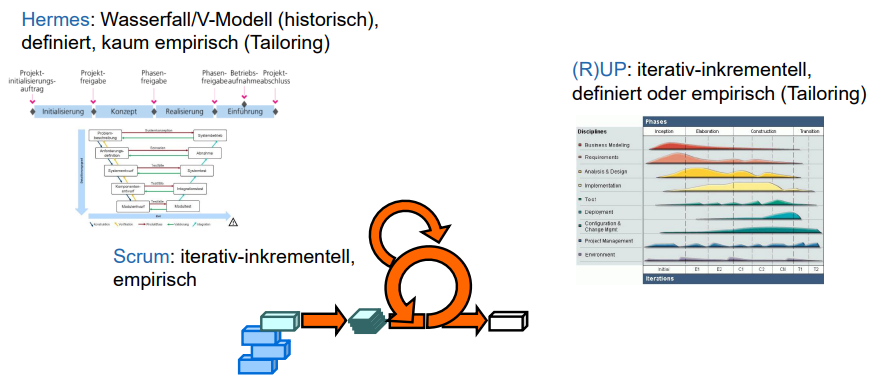
\includegraphics[width=0.3\textwidth]{Resources/Images/CharaktersierungProzessmodellen.png}
\caption{\label{fig:CharaktersierungProzessmodellen}CharaktersierungProzessmodellen}
\end{figure}




















































\end{document}